\documentclass{standalone}
\usepackage{tikz}
\usetikzlibrary{patterns, positioning}

\begin{document}
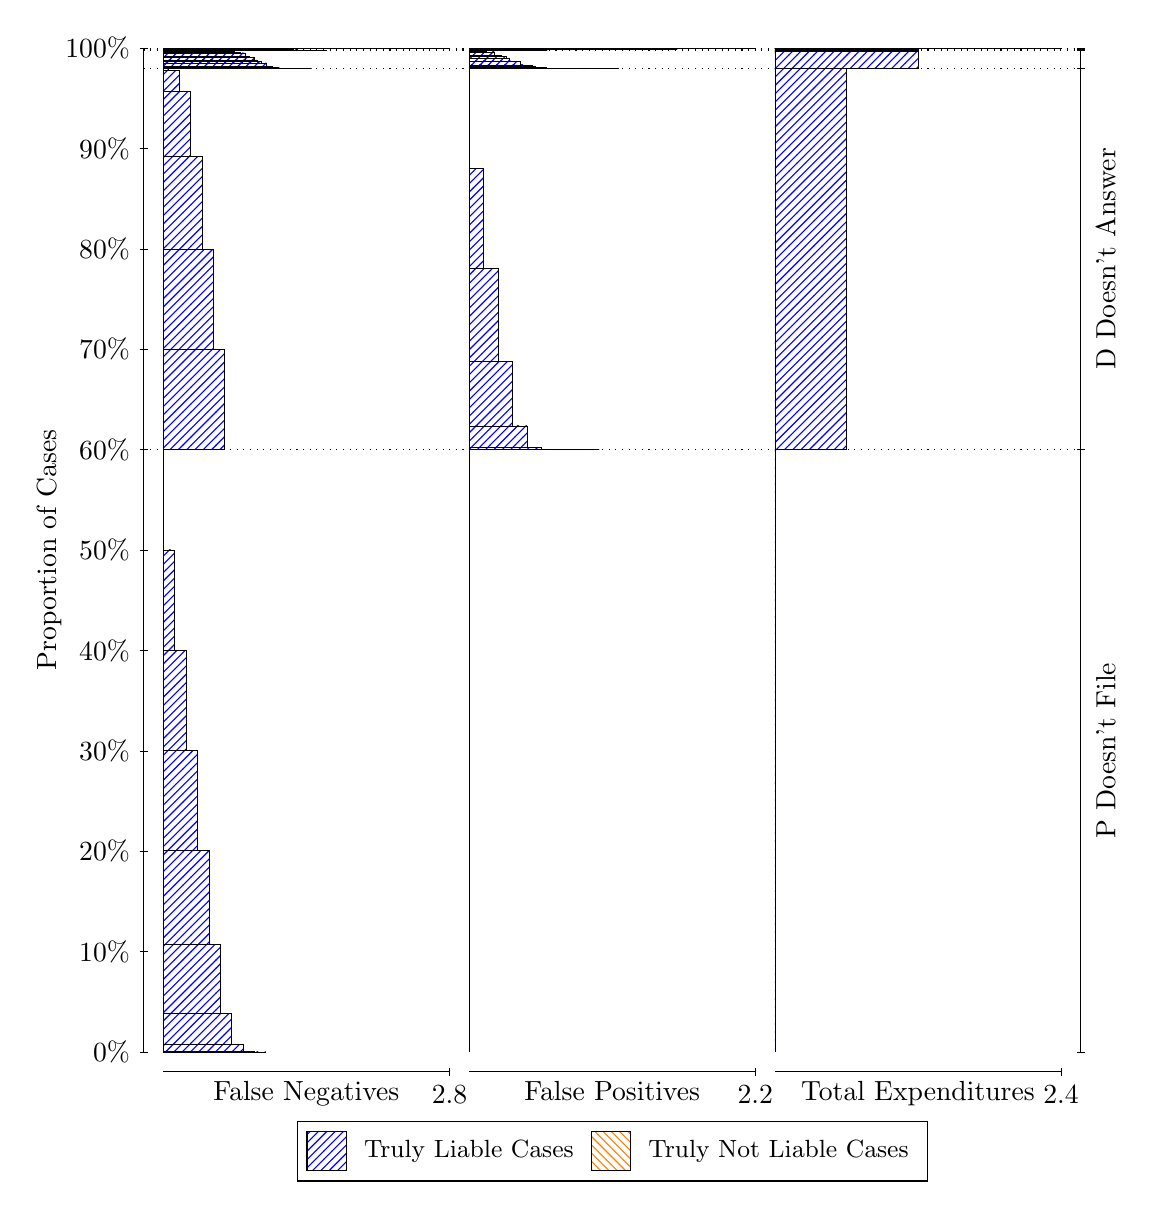
\begin{tikzpicture}
\draw[black, very thin] (1.5,1.75) -- (1.5,14.5);
\node[rotate=90, anchor=center] at (0.3, 8.125) {Proportion of Cases};
\draw[black, very thin] (1.45,1.75) -- (1.55,1.75);
\node[anchor=east] at (1.45, 1.75) {0\%};
\draw[black, very thin] (1.45,3.025) -- (1.55,3.025);
\node[anchor=east] at (1.45, 3.025) {10\%};
\draw[black, very thin] (1.45,4.3) -- (1.55,4.3);
\node[anchor=east] at (1.45, 4.3) {20\%};
\draw[black, very thin] (1.45,5.575) -- (1.55,5.575);
\node[anchor=east] at (1.45, 5.575) {30\%};
\draw[black, very thin] (1.45,6.85) -- (1.55,6.85);
\node[anchor=east] at (1.45, 6.85) {40\%};
\draw[black, very thin] (1.45,8.125) -- (1.55,8.125);
\node[anchor=east] at (1.45, 8.125) {50\%};
\draw[black, very thin] (1.45,9.4) -- (1.55,9.4);
\node[anchor=east] at (1.45, 9.4) {60\%};
\draw[black, very thin] (1.45,10.675) -- (1.55,10.675);
\node[anchor=east] at (1.45, 10.675) {70\%};
\draw[black, very thin] (1.45,11.95) -- (1.55,11.95);
\node[anchor=east] at (1.45, 11.95) {80\%};
\draw[black, very thin] (1.45,13.225) -- (1.55,13.225);
\node[anchor=east] at (1.45, 13.225) {90\%};
\draw[black, very thin] (1.45,14.5) -- (1.55,14.5);
\node[anchor=east] at (1.45, 14.5) {100\%};

\draw[black, very thin] (13.4,1.75) -- (13.4,14.5);
\draw[black, very thin] (13.35,1.75) -- (13.45,1.75);
\node[anchor=west] at (13.35, 1.75) {};
\draw[black, very thin] (13.35,9.4013) -- (13.45,9.4013);
\node[anchor=west] at (13.35, 9.4013) {};
\draw[black, very thin] (13.35,14.245) -- (13.45,14.245);
\node[anchor=west] at (13.35, 14.245) {};
\draw[black, very thin] (13.35,14.474) -- (13.45,14.474);
\node[anchor=west] at (13.35, 14.474) {};
\draw[black, very thin] (13.35,14.488) -- (13.45,14.488);
\node[anchor=west] at (13.35, 14.488) {};
\draw[black, very thin] (13.35,14.495) -- (13.45,14.495);
\node[anchor=west] at (13.35, 14.495) {};
\draw[black, very thin] (13.35,14.5) -- (13.45,14.5);
\node[anchor=west] at (13.35, 14.5) {};

\draw[black, very thin, pattern color=blue, pattern=north east lines] (1.75,1.75) rectangle (3.0476,1.7504);
\draw[black, very thin, pattern color=blue, pattern=north east lines] (1.75,1.7504) rectangle (2.9034,1.7589);
\draw[black, very thin, pattern color=blue, pattern=north east lines] (1.75,1.7589) rectangle (2.7593,1.8446);
\draw[black, very thin, pattern color=blue, pattern=north east lines] (1.75,1.8446) rectangle (2.6151,2.2381);
\draw[black, very thin, pattern color=blue, pattern=north east lines] (1.75,2.2381) rectangle (2.4709,3.1197);
\draw[black, very thin, pattern color=blue, pattern=north east lines] (1.75,3.1197) rectangle (2.3267,4.3095);
\draw[black, very thin, pattern color=blue, pattern=north east lines] (1.75,4.3095) rectangle (2.1825,5.5766);
\draw[black, very thin, pattern color=blue, pattern=north east lines] (1.75,5.5766) rectangle (2.0384,6.8513);
\draw[black, very thin, pattern color=blue, pattern=north east lines] (1.75,6.8513) rectangle (1.8942,8.1263);
\draw[black, very thin, pattern color=orange, pattern=north west lines] (1.75,8.1263) rectangle (1.75,8.1263);
\draw[black, very thin, pattern color=blue, pattern=north east lines] (1.75,8.1263) rectangle (1.75,9.4013);
\draw[black, very thin, pattern color=blue, pattern=north east lines] (1.75,9.4013) rectangle (2.5286,10.676);
\draw[black, very thin, pattern color=blue, pattern=north east lines] (1.75,10.676) rectangle (2.3844,11.942);
\draw[black, very thin, pattern color=blue, pattern=north east lines] (1.75,11.942) rectangle (2.2402,13.124);
\draw[black, very thin, pattern color=blue, pattern=north east lines] (1.75,13.124) rectangle (2.096,13.947);
\draw[black, very thin, pattern color=blue, pattern=north east lines] (1.75,13.947) rectangle (1.9519,14.219);
\draw[black, very thin, pattern color=blue, pattern=north east lines] (1.75,14.219) rectangle (1.8077,14.245);
\draw[black, very thin, pattern color=orange, pattern=north west lines] (1.75,14.245) rectangle (1.75,14.245);
\draw[black, very thin, pattern color=blue, pattern=north east lines] (1.75,14.245) rectangle (1.75,14.245);
\draw[black, very thin, pattern color=blue, pattern=north east lines] (1.75,14.245) rectangle (3.6315,14.245);
\draw[black, very thin, pattern color=blue, pattern=north east lines] (1.75,14.245) rectangle (3.5667,14.245);
\draw[black, very thin, pattern color=blue, pattern=north east lines] (1.75,14.245) rectangle (3.5018,14.245);
\draw[black, very thin, pattern color=blue, pattern=north east lines] (1.75,14.245) rectangle (3.4874,14.245);
\draw[black, very thin, pattern color=blue, pattern=north east lines] (1.75,14.245) rectangle (3.4225,14.245);
\draw[black, very thin, pattern color=blue, pattern=north east lines] (1.75,14.245) rectangle (3.372,14.245);
\draw[black, very thin, pattern color=blue, pattern=north east lines] (1.75,14.245) rectangle (3.3576,14.245);
\draw[black, very thin, pattern color=blue, pattern=north east lines] (1.75,14.245) rectangle (3.3432,14.246);
\draw[black, very thin, pattern color=blue, pattern=north east lines] (1.75,14.246) rectangle (3.3071,14.246);
\draw[black, very thin, pattern color=blue, pattern=north east lines] (1.75,14.246) rectangle (3.2783,14.247);
\draw[black, very thin, pattern color=blue, pattern=north east lines] (1.75,14.247) rectangle (3.2278,14.247);
\draw[black, very thin, pattern color=blue, pattern=north east lines] (1.75,14.247) rectangle (3.2134,14.247);
\draw[black, very thin, pattern color=blue, pattern=north east lines] (1.75,14.247) rectangle (3.199,14.259);
\draw[black, very thin, pattern color=blue, pattern=north east lines] (1.75,14.259) rectangle (3.163,14.259);
\draw[black, very thin, pattern color=blue, pattern=north east lines] (1.75,14.259) rectangle (3.1341,14.268);
\draw[black, very thin, pattern color=blue, pattern=north east lines] (1.75,14.268) rectangle (3.1125,14.268);
\draw[black, very thin, pattern color=blue, pattern=north east lines] (1.75,14.268) rectangle (3.0837,14.269);
\draw[black, very thin, pattern color=blue, pattern=north east lines] (1.75,14.269) rectangle (3.0692,14.27);
\draw[black, very thin, pattern color=blue, pattern=north east lines] (1.75,14.27) rectangle (3.0548,14.31);
\draw[black, very thin, pattern color=blue, pattern=north east lines] (1.75,14.31) rectangle (3.0188,14.31);
\draw[black, very thin, pattern color=blue, pattern=north east lines] (1.75,14.31) rectangle (2.9899,14.33);
\draw[black, very thin, pattern color=blue, pattern=north east lines] (1.75,14.33) rectangle (2.9683,14.331);
\draw[black, very thin, pattern color=blue, pattern=north east lines] (1.75,14.331) rectangle (2.9395,14.349);
\draw[black, very thin, pattern color=blue, pattern=north east lines] (1.75,14.349) rectangle (2.9251,14.349);
\draw[black, very thin, pattern color=blue, pattern=north east lines] (1.75,14.349) rectangle (2.9106,14.381);
\draw[black, very thin, pattern color=blue, pattern=north east lines] (1.75,14.381) rectangle (2.8746,14.382);
\draw[black, very thin, pattern color=blue, pattern=north east lines] (1.75,14.382) rectangle (2.8458,14.39);
\draw[black, very thin, pattern color=blue, pattern=north east lines] (1.75,14.39) rectangle (2.8241,14.392);
\draw[black, very thin, pattern color=blue, pattern=north east lines] (1.75,14.392) rectangle (2.7953,14.433);
\draw[black, very thin, pattern color=blue, pattern=north east lines] (1.75,14.433) rectangle (2.7809,14.433);
\draw[black, very thin, pattern color=blue, pattern=north east lines] (1.75,14.433) rectangle (2.7665,14.439);
\draw[black, very thin, pattern color=blue, pattern=north east lines] (1.75,14.439) rectangle (2.7304,14.44);
\draw[black, very thin, pattern color=blue, pattern=north east lines] (1.75,14.44) rectangle (2.7016,14.441);
\draw[black, very thin, pattern color=blue, pattern=north east lines] (1.75,14.441) rectangle (2.68,14.449);
\draw[black, very thin, pattern color=blue, pattern=north east lines] (1.75,14.449) rectangle (2.6511,14.465);
\draw[black, very thin, pattern color=blue, pattern=north east lines] (1.75,14.465) rectangle (2.6367,14.465);
\draw[black, very thin, pattern color=blue, pattern=north east lines] (1.75,14.465) rectangle (2.6223,14.465);
\draw[black, very thin, pattern color=blue, pattern=north east lines] (1.75,14.465) rectangle (2.5862,14.465);
\draw[black, very thin, pattern color=blue, pattern=north east lines] (1.75,14.465) rectangle (2.5574,14.465);
\draw[black, very thin, pattern color=blue, pattern=north east lines] (1.75,14.465) rectangle (2.5358,14.472);
\draw[black, very thin, pattern color=blue, pattern=north east lines] (1.75,14.472) rectangle (2.5069,14.473);
\draw[black, very thin, pattern color=blue, pattern=north east lines] (1.75,14.473) rectangle (2.4925,14.473);
\draw[black, very thin, pattern color=blue, pattern=north east lines] (1.75,14.473) rectangle (2.4781,14.473);
\draw[black, very thin, pattern color=blue, pattern=north east lines] (1.75,14.473) rectangle (2.4421,14.473);
\draw[black, very thin, pattern color=blue, pattern=north east lines] (1.75,14.473) rectangle (2.4132,14.473);
\draw[black, very thin, pattern color=blue, pattern=north east lines] (1.75,14.473) rectangle (2.3916,14.474);
\draw[black, very thin, pattern color=blue, pattern=north east lines] (1.75,14.474) rectangle (2.3628,14.474);
\draw[black, very thin, pattern color=blue, pattern=north east lines] (1.75,14.474) rectangle (2.3483,14.474);
\draw[black, very thin, pattern color=blue, pattern=north east lines] (1.75,14.474) rectangle (2.3339,14.474);
\draw[black, very thin, pattern color=blue, pattern=north east lines] (1.75,14.474) rectangle (2.2979,14.474);
\draw[black, very thin, pattern color=blue, pattern=north east lines] (1.75,14.474) rectangle (2.269,14.474);
\draw[black, very thin, pattern color=blue, pattern=north east lines] (1.75,14.474) rectangle (2.2474,14.474);
\draw[black, very thin, pattern color=blue, pattern=north east lines] (1.75,14.474) rectangle (2.2186,14.474);
\draw[black, very thin, pattern color=blue, pattern=north east lines] (1.75,14.474) rectangle (2.2042,14.474);
\draw[black, very thin, pattern color=blue, pattern=north east lines] (1.75,14.474) rectangle (2.1537,14.474);
\draw[black, very thin, pattern color=blue, pattern=north east lines] (1.75,14.474) rectangle (2.1032,14.474);
\draw[black, very thin, pattern color=blue, pattern=north east lines] (1.75,14.474) rectangle (2.0744,14.474);
\draw[black, very thin, pattern color=blue, pattern=north east lines] (1.75,14.474) rectangle (2.0095,14.474);
\draw[black, very thin, pattern color=blue, pattern=north east lines] (1.75,14.474) rectangle (1.9591,14.474);
\draw[black, very thin, pattern color=blue, pattern=north east lines] (1.75,14.474) rectangle (1.8149,14.474);
\draw[black, very thin, pattern color=orange, pattern=north west lines] (1.75,14.474) rectangle (1.75,14.474);
\draw[black, very thin, pattern color=blue, pattern=north east lines] (1.75,14.474) rectangle (3.8262,14.474);
\draw[black, very thin, pattern color=blue, pattern=north east lines] (1.75,14.474) rectangle (3.682,14.474);
\draw[black, very thin, pattern color=blue, pattern=north east lines] (1.75,14.474) rectangle (3.5378,14.475);
\draw[black, very thin, pattern color=blue, pattern=north east lines] (1.75,14.475) rectangle (3.3937,14.479);
\draw[black, very thin, pattern color=blue, pattern=north east lines] (1.75,14.479) rectangle (3.2495,14.486);
\draw[black, very thin, pattern color=blue, pattern=north east lines] (1.75,14.486) rectangle (3.1053,14.488);
\draw[black, very thin, pattern color=blue, pattern=north east lines] (1.75,14.488) rectangle (2.9611,14.488);
\draw[black, very thin, pattern color=blue, pattern=north east lines] (1.75,14.488) rectangle (2.8169,14.488);
\draw[black, very thin, pattern color=blue, pattern=north east lines] (1.75,14.488) rectangle (2.6728,14.488);
\draw[black, very thin, pattern color=blue, pattern=north east lines] (1.75,14.488) rectangle (2.5286,14.488);
\draw[black, very thin, pattern color=orange, pattern=north west lines] (1.75,14.488) rectangle (1.75,14.488);
\draw[black, very thin, pattern color=blue, pattern=north east lines] (1.75,14.488) rectangle (2.5286,14.488);
\draw[black, very thin, pattern color=blue, pattern=north east lines] (1.75,14.488) rectangle (2.3844,14.488);
\draw[black, very thin, pattern color=blue, pattern=north east lines] (1.75,14.488) rectangle (2.2402,14.489);
\draw[black, very thin, pattern color=blue, pattern=north east lines] (1.75,14.489) rectangle (2.096,14.492);
\draw[black, very thin, pattern color=blue, pattern=north east lines] (1.75,14.492) rectangle (1.9519,14.494);
\draw[black, very thin, pattern color=blue, pattern=north east lines] (1.75,14.494) rectangle (1.8077,14.495);
\draw[black, very thin, pattern color=orange, pattern=north west lines] (1.75,14.495) rectangle (1.75,14.495);
\draw[black, very thin, pattern color=blue, pattern=north east lines] (1.75,14.495) rectangle (1.75,14.495);
\draw[black, very thin, pattern color=blue, pattern=north east lines] (1.75,14.495) rectangle (5.3833,14.495);
\draw[black, very thin, pattern color=blue, pattern=north east lines] (1.75,14.495) rectangle (5.2392,14.495);
\draw[black, very thin, pattern color=blue, pattern=north east lines] (1.75,14.495) rectangle (5.095,14.495);
\draw[black, very thin, pattern color=blue, pattern=north east lines] (1.75,14.495) rectangle (4.9508,14.495);
\draw[black, very thin, pattern color=blue, pattern=north east lines] (1.75,14.495) rectangle (4.8066,14.495);
\draw[black, very thin, pattern color=blue, pattern=north east lines] (1.75,14.495) rectangle (4.6624,14.495);
\draw[black, very thin, pattern color=blue, pattern=north east lines] (1.75,14.495) rectangle (4.6624,14.495);
\draw[black, very thin, pattern color=blue, pattern=north east lines] (1.75,14.495) rectangle (4.5183,14.495);
\draw[black, very thin, pattern color=blue, pattern=north east lines] (1.75,14.495) rectangle (4.5183,14.495);
\draw[black, very thin, pattern color=blue, pattern=north east lines] (1.75,14.495) rectangle (4.3741,14.495);
\draw[black, very thin, pattern color=blue, pattern=north east lines] (1.75,14.495) rectangle (4.3164,14.495);
\draw[black, very thin, pattern color=blue, pattern=north east lines] (1.75,14.495) rectangle (4.2299,14.495);
\draw[black, very thin, pattern color=blue, pattern=north east lines] (1.75,14.495) rectangle (4.2299,14.495);
\draw[black, very thin, pattern color=blue, pattern=north east lines] (1.75,14.495) rectangle (4.1722,14.495);
\draw[black, very thin, pattern color=blue, pattern=north east lines] (1.75,14.495) rectangle (4.0857,14.495);
\draw[black, very thin, pattern color=blue, pattern=north east lines] (1.75,14.495) rectangle (4.028,14.495);
\draw[black, very thin, pattern color=blue, pattern=north east lines] (1.75,14.495) rectangle (3.9415,14.495);
\draw[black, very thin, pattern color=blue, pattern=north east lines] (1.75,14.495) rectangle (3.8839,14.495);
\draw[black, very thin, pattern color=blue, pattern=north east lines] (1.75,14.495) rectangle (3.7974,14.495);
\draw[black, very thin, pattern color=blue, pattern=north east lines] (1.75,14.495) rectangle (3.7397,14.495);
\draw[black, very thin, pattern color=blue, pattern=north east lines] (1.75,14.495) rectangle (3.5955,14.495);
\draw[black, very thin, pattern color=blue, pattern=north east lines] (1.75,14.495) rectangle (3.5955,14.496);
\draw[black, very thin, pattern color=blue, pattern=north east lines] (1.75,14.496) rectangle (3.4513,14.496);
\draw[black, very thin, pattern color=blue, pattern=north east lines] (1.75,14.496) rectangle (3.4513,14.497);
\draw[black, very thin, pattern color=blue, pattern=north east lines] (1.75,14.497) rectangle (3.3071,14.498);
\draw[black, very thin, pattern color=blue, pattern=north east lines] (1.75,14.498) rectangle (3.163,14.499);
\draw[black, very thin, pattern color=blue, pattern=north east lines] (1.75,14.499) rectangle (3.163,14.499);
\draw[black, very thin, pattern color=blue, pattern=north east lines] (1.75,14.499) rectangle (3.0188,14.499);
\draw[black, very thin, pattern color=blue, pattern=north east lines] (1.75,14.499) rectangle (3.0188,14.5);
\draw[black, very thin, pattern color=blue, pattern=north east lines] (1.75,14.5) rectangle (3.0188,14.5);
\draw[black, very thin, pattern color=blue, pattern=north east lines] (1.75,14.5) rectangle (2.8746,14.5);
\draw[black, very thin, pattern color=blue, pattern=north east lines] (1.75,14.5) rectangle (2.8746,14.5);
\draw[black, very thin, pattern color=blue, pattern=north east lines] (1.75,14.5) rectangle (2.7304,14.5);
\draw[black, very thin, pattern color=blue, pattern=north east lines] (1.75,14.5) rectangle (2.5862,14.5);
\draw[black, very thin, pattern color=blue, pattern=north east lines] (1.75,14.5) rectangle (2.4421,14.5);
\draw[black, very thin, pattern color=blue, pattern=north east lines] (1.75,14.5) rectangle (2.4421,14.5);
\draw[black, very thin, pattern color=blue, pattern=north east lines] (1.75,14.5) rectangle (2.2979,14.5);
\draw[black, very thin, pattern color=blue, pattern=north east lines] (1.75,14.5) rectangle (2.2979,14.5);
\draw[black, very thin, pattern color=blue, pattern=north east lines] (1.75,14.5) rectangle (2.1537,14.5);
\draw[black, very thin, pattern color=blue, pattern=north east lines] (1.75,14.5) rectangle (2.1537,14.5);
\draw[black, very thin, pattern color=blue, pattern=north east lines] (1.75,14.5) rectangle (2.0095,14.5);
\draw[black, very thin, pattern color=orange, pattern=north west lines] (1.75,14.5) rectangle (1.75,14.5);
\draw[black, very thin, pattern color=orange, pattern=north west lines] (5.6333,1.75) rectangle (5.6333,1.75);
\draw[black, very thin, pattern color=blue, pattern=north east lines] (5.6333,1.75) rectangle (5.6333,9.4013);
\draw[black, very thin, pattern color=orange, pattern=north west lines] (5.6333,9.4013) rectangle (7.2848,9.4013);
\draw[black, very thin, pattern color=blue, pattern=north east lines] (5.6333,9.4013) rectangle (7.2848,9.4013);
\draw[black, very thin, pattern color=blue, pattern=north east lines] (5.6333,9.4013) rectangle (7.1013,9.4013);
\draw[black, very thin, pattern color=blue, pattern=north east lines] (5.6333,9.4013) rectangle (6.9178,9.4013);
\draw[black, very thin, pattern color=blue, pattern=north east lines] (5.6333,9.4013) rectangle (6.7343,9.4018);
\draw[black, very thin, pattern color=blue, pattern=north east lines] (5.6333,9.4018) rectangle (6.5508,9.4281);
\draw[black, very thin, pattern color=blue, pattern=north east lines] (5.6333,9.4281) rectangle (6.3673,9.7001);
\draw[black, very thin, pattern color=blue, pattern=north east lines] (5.6333,9.7001) rectangle (6.1838,10.523);
\draw[black, very thin, pattern color=blue, pattern=north east lines] (5.6333,10.523) rectangle (6.0003,11.705);
\draw[black, very thin, pattern color=blue, pattern=north east lines] (5.6333,11.705) rectangle (5.8168,12.971);
\draw[black, very thin, pattern color=blue, pattern=north east lines] (5.6333,12.971) rectangle (5.6333,14.245);
\draw[black, very thin, pattern color=orange, pattern=north west lines] (5.6333,14.245) rectangle (7.5326,14.245);
\draw[black, very thin, pattern color=blue, pattern=north east lines] (5.6333,14.245) rectangle (7.5326,14.245);
\draw[black, very thin, pattern color=blue, pattern=north east lines] (5.6333,14.245) rectangle (7.3491,14.245);
\draw[black, very thin, pattern color=orange, pattern=north west lines] (5.6333,14.245) rectangle (7.2848,14.245);
\draw[black, very thin, pattern color=blue, pattern=north east lines] (5.6333,14.245) rectangle (7.2848,14.245);
\draw[black, very thin, pattern color=orange, pattern=north west lines] (5.6333,14.245) rectangle (7.2023,14.245);
\draw[black, very thin, pattern color=blue, pattern=north east lines] (5.6333,14.245) rectangle (7.2023,14.245);
\draw[black, very thin, pattern color=blue, pattern=north east lines] (5.6333,14.245) rectangle (7.1656,14.245);
\draw[black, very thin, pattern color=blue, pattern=north east lines] (5.6333,14.245) rectangle (7.1013,14.245);
\draw[black, very thin, pattern color=orange, pattern=north west lines] (5.6333,14.245) rectangle (7.0371,14.245);
\draw[black, very thin, pattern color=blue, pattern=north east lines] (5.6333,14.245) rectangle (7.0371,14.245);
\draw[black, very thin, pattern color=blue, pattern=north east lines] (5.6333,14.245) rectangle (7.0188,14.245);
\draw[black, very thin, pattern color=blue, pattern=north east lines] (5.6333,14.245) rectangle (6.9821,14.245);
\draw[black, very thin, pattern color=orange, pattern=north west lines] (5.6333,14.245) rectangle (6.9545,14.245);
\draw[black, very thin, pattern color=blue, pattern=north east lines] (5.6333,14.245) rectangle (6.9545,14.245);
\draw[black, very thin, pattern color=blue, pattern=north east lines] (5.6333,14.245) rectangle (6.9178,14.245);
\draw[black, very thin, pattern color=orange, pattern=north west lines] (5.6333,14.245) rectangle (6.872,14.245);
\draw[black, very thin, pattern color=blue, pattern=north east lines] (5.6333,14.245) rectangle (6.872,14.245);
\draw[black, very thin, pattern color=blue, pattern=north east lines] (5.6333,14.245) rectangle (6.8536,14.245);
\draw[black, very thin, pattern color=blue, pattern=north east lines] (5.6333,14.245) rectangle (6.8353,14.245);
\draw[black, very thin, pattern color=blue, pattern=north east lines] (5.6333,14.245) rectangle (6.7986,14.246);
\draw[black, very thin, pattern color=blue, pattern=north east lines] (5.6333,14.246) rectangle (6.771,14.246);
\draw[black, very thin, pattern color=blue, pattern=north east lines] (5.6333,14.246) rectangle (6.7343,14.246);
\draw[black, very thin, pattern color=blue, pattern=north east lines] (5.6333,14.246) rectangle (6.6885,14.246);
\draw[black, very thin, pattern color=blue, pattern=north east lines] (5.6333,14.246) rectangle (6.6701,14.246);
\draw[black, very thin, pattern color=blue, pattern=north east lines] (5.6333,14.246) rectangle (6.6518,14.247);
\draw[black, very thin, pattern color=blue, pattern=north east lines] (5.6333,14.247) rectangle (6.6151,14.254);
\draw[black, very thin, pattern color=blue, pattern=north east lines] (5.6333,14.254) rectangle (6.5875,14.254);
\draw[black, very thin, pattern color=blue, pattern=north east lines] (5.6333,14.254) rectangle (6.5508,14.254);
\draw[black, very thin, pattern color=blue, pattern=north east lines] (5.6333,14.254) rectangle (6.505,14.254);
\draw[black, very thin, pattern color=blue, pattern=north east lines] (5.6333,14.254) rectangle (6.4866,14.254);
\draw[black, very thin, pattern color=blue, pattern=north east lines] (5.6333,14.254) rectangle (6.4683,14.27);
\draw[black, very thin, pattern color=blue, pattern=north east lines] (5.6333,14.27) rectangle (6.4316,14.278);
\draw[black, very thin, pattern color=blue, pattern=north east lines] (5.6333,14.278) rectangle (6.404,14.279);
\draw[black, very thin, pattern color=blue, pattern=north east lines] (5.6333,14.279) rectangle (6.3673,14.28);
\draw[black, very thin, pattern color=blue, pattern=north east lines] (5.6333,14.28) rectangle (6.3215,14.286);
\draw[black, very thin, pattern color=blue, pattern=north east lines] (5.6333,14.286) rectangle (6.3031,14.286);
\draw[black, very thin, pattern color=blue, pattern=north east lines] (5.6333,14.286) rectangle (6.2848,14.327);
\draw[black, very thin, pattern color=blue, pattern=north east lines] (5.6333,14.327) rectangle (6.2481,14.329);
\draw[black, very thin, pattern color=blue, pattern=north east lines] (5.6333,14.329) rectangle (6.2205,14.337);
\draw[black, very thin, pattern color=blue, pattern=north east lines] (5.6333,14.337) rectangle (6.1838,14.338);
\draw[black, very thin, pattern color=blue, pattern=north east lines] (5.6333,14.338) rectangle (6.138,14.37);
\draw[black, very thin, pattern color=blue, pattern=north east lines] (5.6333,14.37) rectangle (6.1196,14.37);
\draw[black, very thin, pattern color=blue, pattern=north east lines] (5.6333,14.37) rectangle (6.1013,14.389);
\draw[black, very thin, pattern color=blue, pattern=north east lines] (5.6333,14.389) rectangle (6.0646,14.389);
\draw[black, very thin, pattern color=blue, pattern=north east lines] (5.6333,14.389) rectangle (6.037,14.409);
\draw[black, very thin, pattern color=blue, pattern=north east lines] (5.6333,14.409) rectangle (6.0003,14.409);
\draw[black, very thin, pattern color=blue, pattern=north east lines] (5.6333,14.409) rectangle (5.9545,14.45);
\draw[black, very thin, pattern color=blue, pattern=north east lines] (5.6333,14.45) rectangle (5.9361,14.45);
\draw[black, very thin, pattern color=blue, pattern=north east lines] (5.6333,14.45) rectangle (5.9178,14.452);
\draw[black, very thin, pattern color=blue, pattern=north east lines] (5.6333,14.452) rectangle (5.8811,14.452);
\draw[black, very thin, pattern color=blue, pattern=north east lines] (5.6333,14.452) rectangle (5.8535,14.461);
\draw[black, very thin, pattern color=blue, pattern=north east lines] (5.6333,14.461) rectangle (5.8168,14.461);
\draw[black, very thin, pattern color=blue, pattern=north east lines] (5.6333,14.461) rectangle (5.771,14.472);
\draw[black, very thin, pattern color=blue, pattern=north east lines] (5.6333,14.472) rectangle (5.7526,14.472);
\draw[black, very thin, pattern color=blue, pattern=north east lines] (5.6333,14.472) rectangle (5.7343,14.472);
\draw[black, very thin, pattern color=blue, pattern=north east lines] (5.6333,14.472) rectangle (5.67,14.473);
\draw[black, very thin, pattern color=blue, pattern=north east lines] (5.6333,14.473) rectangle (5.6333,14.474);
\draw[black, very thin, pattern color=orange, pattern=north west lines] (5.6333,14.474) rectangle (6.6242,14.474);
\draw[black, very thin, pattern color=blue, pattern=north east lines] (5.6333,14.474) rectangle (6.6242,14.474);
\draw[black, very thin, pattern color=blue, pattern=north east lines] (5.6333,14.474) rectangle (6.4407,14.474);
\draw[black, very thin, pattern color=blue, pattern=north east lines] (5.6333,14.474) rectangle (6.2572,14.474);
\draw[black, very thin, pattern color=blue, pattern=north east lines] (5.6333,14.474) rectangle (6.0737,14.474);
\draw[black, very thin, pattern color=blue, pattern=north east lines] (5.6333,14.474) rectangle (5.8902,14.476);
\draw[black, very thin, pattern color=blue, pattern=north east lines] (5.6333,14.476) rectangle (5.7067,14.482);
\draw[black, very thin, pattern color=blue, pattern=north east lines] (5.6333,14.482) rectangle (5.6333,14.488);
\draw[black, very thin, pattern color=orange, pattern=north west lines] (5.6333,14.488) rectangle (8.2758,14.488);
\draw[black, very thin, pattern color=blue, pattern=north east lines] (5.6333,14.488) rectangle (8.2758,14.488);
\draw[black, very thin, pattern color=blue, pattern=north east lines] (5.6333,14.488) rectangle (8.0923,14.488);
\draw[black, very thin, pattern color=blue, pattern=north east lines] (5.6333,14.488) rectangle (7.9088,14.488);
\draw[black, very thin, pattern color=blue, pattern=north east lines] (5.6333,14.488) rectangle (7.7253,14.488);
\draw[black, very thin, pattern color=blue, pattern=north east lines] (5.6333,14.488) rectangle (7.5418,14.488);
\draw[black, very thin, pattern color=blue, pattern=north east lines] (5.6333,14.488) rectangle (7.3582,14.491);
\draw[black, very thin, pattern color=blue, pattern=north east lines] (5.6333,14.491) rectangle (7.1747,14.494);
\draw[black, very thin, pattern color=blue, pattern=north east lines] (5.6333,14.494) rectangle (6.9912,14.495);
\draw[black, very thin, pattern color=blue, pattern=north east lines] (5.6333,14.495) rectangle (6.8077,14.495);
\draw[black, very thin, pattern color=blue, pattern=north east lines] (5.6333,14.495) rectangle (6.6242,14.495);
\draw[black, very thin, pattern color=orange, pattern=north west lines] (5.6333,14.495) rectangle (9.2667,14.495);
\draw[black, very thin, pattern color=blue, pattern=north east lines] (5.6333,14.495) rectangle (9.2667,14.495);
\draw[black, very thin, pattern color=blue, pattern=north east lines] (5.6333,14.495) rectangle (9.0832,14.495);
\draw[black, very thin, pattern color=orange, pattern=north west lines] (5.6333,14.495) rectangle (9.0832,14.495);
\draw[black, very thin, pattern color=blue, pattern=north east lines] (5.6333,14.495) rectangle (9.0832,14.495);
\draw[black, very thin, pattern color=orange, pattern=north west lines] (5.6333,14.495) rectangle (8.8997,14.495);
\draw[black, very thin, pattern color=blue, pattern=north east lines] (5.6333,14.495) rectangle (8.8997,14.495);
\draw[black, very thin, pattern color=blue, pattern=north east lines] (5.6333,14.495) rectangle (8.8997,14.495);
\draw[black, very thin, pattern color=blue, pattern=north east lines] (5.6333,14.495) rectangle (8.7162,14.495);
\draw[black, very thin, pattern color=orange, pattern=north west lines] (5.6333,14.495) rectangle (8.7162,14.495);
\draw[black, very thin, pattern color=blue, pattern=north east lines] (5.6333,14.495) rectangle (8.7162,14.495);
\draw[black, very thin, pattern color=blue, pattern=north east lines] (5.6333,14.495) rectangle (8.7162,14.495);
\draw[black, very thin, pattern color=blue, pattern=north east lines] (5.6333,14.495) rectangle (8.5327,14.495);
\draw[black, very thin, pattern color=orange, pattern=north west lines] (5.6333,14.495) rectangle (8.5327,14.495);
\draw[black, very thin, pattern color=blue, pattern=north east lines] (5.6333,14.495) rectangle (8.5327,14.495);
\draw[black, very thin, pattern color=blue, pattern=north east lines] (5.6333,14.495) rectangle (8.5327,14.495);
\draw[black, very thin, pattern color=blue, pattern=north east lines] (5.6333,14.495) rectangle (8.3492,14.495);
\draw[black, very thin, pattern color=orange, pattern=north west lines] (5.6333,14.495) rectangle (8.3492,14.495);
\draw[black, very thin, pattern color=blue, pattern=north east lines] (5.6333,14.495) rectangle (8.3492,14.495);
\draw[black, very thin, pattern color=blue, pattern=north east lines] (5.6333,14.495) rectangle (8.3492,14.495);
\draw[black, very thin, pattern color=blue, pattern=north east lines] (5.6333,14.495) rectangle (8.1657,14.495);
\draw[black, very thin, pattern color=blue, pattern=north east lines] (5.6333,14.495) rectangle (8.1657,14.495);
\draw[black, very thin, pattern color=orange, pattern=north west lines] (5.6333,14.495) rectangle (8.1657,14.495);
\draw[black, very thin, pattern color=blue, pattern=north east lines] (5.6333,14.495) rectangle (8.1657,14.495);
\draw[black, very thin, pattern color=blue, pattern=north east lines] (5.6333,14.495) rectangle (8.1657,14.495);
\draw[black, very thin, pattern color=blue, pattern=north east lines] (5.6333,14.495) rectangle (7.9822,14.495);
\draw[black, very thin, pattern color=blue, pattern=north east lines] (5.6333,14.495) rectangle (7.9822,14.495);
\draw[black, very thin, pattern color=orange, pattern=north west lines] (5.6333,14.495) rectangle (7.9822,14.495);
\draw[black, very thin, pattern color=blue, pattern=north east lines] (5.6333,14.495) rectangle (7.9822,14.496);
\draw[black, very thin, pattern color=blue, pattern=north east lines] (5.6333,14.496) rectangle (7.7987,14.496);
\draw[black, very thin, pattern color=blue, pattern=north east lines] (5.6333,14.496) rectangle (7.7987,14.497);
\draw[black, very thin, pattern color=blue, pattern=north east lines] (5.6333,14.497) rectangle (7.7987,14.497);
\draw[black, very thin, pattern color=blue, pattern=north east lines] (5.6333,14.497) rectangle (7.6152,14.497);
\draw[black, very thin, pattern color=blue, pattern=north east lines] (5.6333,14.497) rectangle (7.6152,14.498);
\draw[black, very thin, pattern color=blue, pattern=north east lines] (5.6333,14.498) rectangle (7.6152,14.498);
\draw[black, very thin, pattern color=blue, pattern=north east lines] (5.6333,14.498) rectangle (7.4316,14.499);
\draw[black, very thin, pattern color=blue, pattern=north east lines] (5.6333,14.499) rectangle (7.4316,14.499);
\draw[black, very thin, pattern color=blue, pattern=north east lines] (5.6333,14.499) rectangle (7.4316,14.499);
\draw[black, very thin, pattern color=blue, pattern=north east lines] (5.6333,14.499) rectangle (7.2481,14.499);
\draw[black, very thin, pattern color=blue, pattern=north east lines] (5.6333,14.499) rectangle (7.2481,14.499);
\draw[black, very thin, pattern color=blue, pattern=north east lines] (5.6333,14.499) rectangle (7.2481,14.5);
\draw[black, very thin, pattern color=blue, pattern=north east lines] (5.6333,14.5) rectangle (7.0646,14.5);
\draw[black, very thin, pattern color=blue, pattern=north east lines] (5.6333,14.5) rectangle (7.0646,14.5);
\draw[black, very thin, pattern color=blue, pattern=north east lines] (5.6333,14.5) rectangle (7.0646,14.5);
\draw[black, very thin, pattern color=orange, pattern=north west lines] (5.6333,14.5) rectangle (6.9912,14.5);
\draw[black, very thin, pattern color=blue, pattern=north east lines] (5.6333,14.5) rectangle (6.9912,14.5);
\draw[black, very thin, pattern color=blue, pattern=north east lines] (5.6333,14.5) rectangle (6.8811,14.5);
\draw[black, very thin, pattern color=blue, pattern=north east lines] (5.6333,14.5) rectangle (6.8811,14.5);
\draw[black, very thin, pattern color=orange, pattern=north west lines] (5.6333,14.5) rectangle (6.8077,14.5);
\draw[black, very thin, pattern color=blue, pattern=north east lines] (5.6333,14.5) rectangle (6.8077,14.5);
\draw[black, very thin, pattern color=blue, pattern=north east lines] (5.6333,14.5) rectangle (6.6976,14.5);
\draw[black, very thin, pattern color=blue, pattern=north east lines] (5.6333,14.5) rectangle (6.6976,14.5);
\draw[black, very thin, pattern color=orange, pattern=north west lines] (5.6333,14.5) rectangle (6.6242,14.5);
\draw[black, very thin, pattern color=blue, pattern=north east lines] (5.6333,14.5) rectangle (6.6242,14.5);
\draw[black, very thin, pattern color=blue, pattern=north east lines] (5.6333,14.5) rectangle (6.6242,14.5);
\draw[black, very thin, pattern color=blue, pattern=north east lines] (5.6333,14.5) rectangle (6.5141,14.5);
\draw[black, very thin, pattern color=blue, pattern=north east lines] (5.6333,14.5) rectangle (6.4407,14.5);
\draw[black, very thin, pattern color=blue, pattern=north east lines] (5.6333,14.5) rectangle (6.4407,14.5);
\draw[black, very thin, pattern color=blue, pattern=north east lines] (5.6333,14.5) rectangle (6.3306,14.5);
\draw[black, very thin, pattern color=blue, pattern=north east lines] (5.6333,14.5) rectangle (6.2572,14.5);
\draw[black, very thin, pattern color=blue, pattern=north east lines] (5.6333,14.5) rectangle (6.2572,14.5);
\draw[black, very thin, pattern color=blue, pattern=north east lines] (5.6333,14.5) rectangle (6.0737,14.5);
\draw[black, very thin, pattern color=blue, pattern=north east lines] (5.6333,14.5) rectangle (6.0737,14.5);
\draw[black, very thin, pattern color=blue, pattern=north east lines] (5.6333,14.5) rectangle (5.8902,14.5);
\draw[black, very thin, pattern color=blue, pattern=north east lines] (5.6333,14.5) rectangle (5.8902,14.5);
\draw[black, very thin, pattern color=blue, pattern=north east lines] (5.6333,14.5) rectangle (5.7067,14.5);
\draw[black, very thin, pattern color=blue, pattern=north east lines] (5.6333,14.5) rectangle (5.6333,14.5);
\draw[black, very thin, pattern color=orange, pattern=north west lines] (9.5167,1.75) rectangle (9.5167,1.75);
\draw[black, very thin, pattern color=blue, pattern=north east lines] (9.5167,1.75) rectangle (9.5167,9.4013);
\draw[black, very thin, pattern color=orange, pattern=north west lines] (9.5167,9.4013) rectangle (10.425,9.4013);
\draw[black, very thin, pattern color=blue, pattern=north east lines] (9.5167,9.4013) rectangle (10.425,14.245);
\draw[black, very thin, pattern color=orange, pattern=north west lines] (9.5167,14.245) rectangle (11.333,14.245);
\draw[black, very thin, pattern color=blue, pattern=north east lines] (9.5167,14.245) rectangle (11.333,14.456);
\draw[black, very thin, pattern color=orange, pattern=north west lines] (9.5167,14.456) rectangle (11.333,14.456);
\draw[black, very thin, pattern color=blue, pattern=north east lines] (9.5167,14.456) rectangle (11.333,14.474);
\draw[black, very thin, pattern color=orange, pattern=north west lines] (9.5167,14.474) rectangle (11.333,14.474);
\draw[black, very thin, pattern color=blue, pattern=north east lines] (9.5167,14.474) rectangle (11.333,14.488);
\draw[black, very thin, pattern color=orange, pattern=north west lines] (9.5167,14.488) rectangle (11.333,14.488);
\draw[black, very thin, pattern color=blue, pattern=north east lines] (9.5167,14.488) rectangle (11.333,14.495);
\draw[black, very thin, pattern color=orange, pattern=north west lines] (9.5167,14.495) rectangle (13.15,14.495);
\draw[black, very thin, pattern color=blue, pattern=north east lines] (9.5167,14.495) rectangle (13.15,14.495);
\draw[black, very thin, pattern color=orange, pattern=north west lines] (9.5167,14.495) rectangle (13.15,14.495);
\draw[black, very thin, pattern color=blue, pattern=north east lines] (9.5167,14.495) rectangle (13.15,14.499);
\draw[black, very thin, pattern color=orange, pattern=north west lines] (9.5167,14.499) rectangle (13.15,14.499);
\draw[black, very thin, pattern color=blue, pattern=north east lines] (9.5167,14.499) rectangle (13.15,14.5);
\draw[black, dotted] (1.5,9.4013) -- (13.4,9.4013);
\draw[black, dotted] (1.5,14.245) -- (13.4,14.245);
\draw[black, dotted] (1.5,14.474) -- (13.4,14.474);
\draw[black, dotted] (1.5,14.488) -- (13.4,14.488);
\draw[black, dotted] (1.5,14.495) -- (13.4,14.495);
\draw[black, very thin] (1.75,1.5) -- (5.3833,1.5);
\node[anchor=north] at (3.5667, 1.5) {False Negatives};
\draw[black, very thin] (5.3833,1.45) -- (5.3833,1.55);
\node[anchor=north] at (5.3833, 1.45) {2.8};

\draw[black, very thin] (5.6333,1.5) -- (9.2667,1.5);
\node[anchor=north] at (7.45, 1.5) {False Positives};
\draw[black, very thin] (9.2667,1.45) -- (9.2667,1.55);
\node[anchor=north] at (9.2667, 1.45) {2.2};

\draw[black, very thin] (9.5167,1.5) -- (13.15,1.5);
\node[anchor=north] at (11.333, 1.5) {Total Expenditures};
\draw[black, very thin] (13.15,1.45) -- (13.15,1.55);
\node[anchor=north] at (13.15, 1.45) {2.4};

\node[black, centered, rotate=90] at (13.72, 5.5756) {P Doesn't File};
\node[black, centered, rotate=90] at (13.72, 11.823) {D Doesn't Answer};





\draw (7.449999999999999,1.5) node[draw=none] (baseCoordinate) {};
\begin{scope}[align=center]
        \matrix[scale=0.5, draw=black, below=0.5cm of baseCoordinate, nodes={draw}, column sep=0.1cm]{
            \node[rectangle, draw, minimum width=0.5cm, minimum height=0.5cm, pattern=north east lines, pattern color=blue] {}; &
            \node[draw=none, font=\small] (B) {Truly Liable Cases}; &
            \node[rectangle, draw, minimum width=0.5cm, minimum height=0.5cm, pattern=north west lines, pattern color=orange] {}; &
            \node[draw=none, font=\small] (B) {Truly Not Liable Cases}; \\
            };
\end{scope}

\end{tikzpicture}
\end{document}